PETALO is a clear case of direct transference of the technology developed in the context of an experiment related with fundamental research in particle physics (the search for neutrinoless double beta processes), to a medical imaging application with the potential of leading the field in several aspects (energy resolution, full 3D imagining within the detectors, capability of resolving Compton interaction, excellent time resolution providing unsurpassed TOF capabilities and compatibility with NMR).  

The previous work of the teams participating in this proposal, relevant to this project, can be summarised as follows:

\paragraph{IFIC group: technology transfer from the NEXT collaboration}

The \emph{Neutrino Experiment with a Xenon TPC} (NEXT)\footnote{http://next.ific.uv.es/next/} will search for neutrinoless double beta decay processes (\bbonu) in \XE\ using a  high-pressure xenon gas time projection chamber. The design of the NEW (the first stage of the experiment, deploying 10 kg of enriched xenon) and NEXT-100 (second stage, deploying 100 kg of \XE) detectors is optimised for energy resolution by using proportional electroluminescent (EL) amplification of the ionisation signal. The detection of EL light provides an energy measurement using photomultipliers (PMTs) located behind the cathode (the \emph{energy plane}) as well as tracking through its detection a few mm away from production at the anode, via a dense array of silicon photomultipliers (the \emph{tracking plane}).

\begin{figure}[!htb]
	\centering
	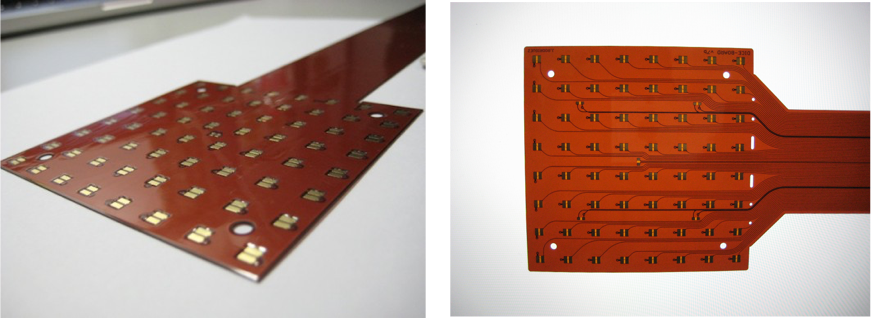
\includegraphics[scale=0.9]{img/KDB2.png}\\
	\caption{\label{fig.KDB} Top and bottom pictures of the Kapton Dice Boards (KDB) developed for the tracking plane of the NEW and NEXT-100 detectors by the NEXT collaboration.}
\end{figure}

In NEW and NEXT-100 the tracking function is provided by a plane of SiPMs operating as light-pixels and located behind the transparent EL grids. They are mounted on flexible radiopure Kapton Dice Boards (KDBs). Each KDB hosts 64 SiPMs (Figure  \ref{ffig.KDB}). The NEW  tracking plane is currently being commissioned with 28 KDBs. The NEXT-100 tracking plane will deploy 112 KDBs.  

The dice boards for the LXSC will be built using the technology developed by NEXT. The design is essentially the same, since the SiPMs foreseen for PETALO are of the same type deployed by NEW and NEXT-100 (SENSL C or J series). The main difference is the size of the SIPM (6 mm rather than 1 mm) which however affects very little the design. 

The NEXT KDBs have been developed by the IFIC group during a period of five years. Currently the technology and expertise of the group is very mature. Furthermore, the two leading electronics engineers working in the NEXT tracking plane (J. Rodríguez and V. Álvarez) have obtained 3-year contracts as ``support technicians" (técnicos de apoyo) to work at IFIC. Given the fact that the NEW tracking plane has been completed and the construction of the NEXT-100 tracking plane will not start until 2017 (2016 will be devoted to running NEW in order to fully validate the technology before starting construction of the final detector), both engineers can devote part of their time, during 2016, to the design and production of the PETALO KDBs. 

PETALO is a liquid-xenon, scintillation based detector with a simpler design and operating conditions  that the NEXT-DEMO, NEW and NEXT-100 detectors. It does not operate at high pressure and does not involve electric fields. Cryogeny at LXe temperatures is rather straight forward and the purification of the gas system much simpler than in the case of NEXT. The mechanical design and construction will be done by Alberto Martínez, a mechanical engineer who has been the leading designer in the NEXT project and who has also obtained a 3-year contract as ``técnico de apoyo''. The operation and commissioning of the prototypes will be done by a post-doc hired with funds requested in this project and supervised by the PI of the project (JDM) and by Dr. I. Liubarsky, the technical coordinator of NEXT and an expert bot in xenon gas systems and cryogenic systems (Dr. Liubarsky was a leading physicist in the  ZEPLIN collaboration, which built a pioneer LXe detector for dark matter searchers). 

The simulations of the LXSC and the development of the reconstruction algorithms for the LXSCs are the responsibility of Dr. Paola Ferrario (PF) who will apply to an independent grant (``young researchers'') in Fall, 2015, as well as other grants (e.g, Severo Ochoa post-doc). 

To summarise, the design and construction of the LXSC of PETALO is a direct technology transfer from the NEXT experiment. The availability of three engineers at the IFIC with 3-years contracts as ``support technician'' and sufficient time availability to share their work between NEXT and PETALO, makes the design and construction of the detector realistic. The IFIC group working in PETALO will also benefit from the support of expert physicists in the NEXT group. The project can be developed in the well equipped laboratories at IFIC. The project will have the full dedication of the PI, two post-docs (PF, see above, and a new post-doc for whom funding is requested) and one graduate student (an FPI grant is also requested). 

\paragraph{I3M-UPV group: expertise in the development of ASICS for PET}

\paragraph{IGIBI230-LaFe group: expertise in clinical validation for PET and in PET imaging}